\documentclass[journal]{IEEEtran}

% Basic
\usepackage[utf8]{inputenc}
\usepackage{graphicx}
\usepackage{amsmath,amssymb,mathtools}
\usepackage{cite}
\usepackage{xcolor}
\usepackage{algorithm}
\usepackage{algpseudocode}
\usepackage{float}
\usepackage{multicol}
\usepackage{multirow}
\usepackage{footmisc}
\usepackage{stackengine}
\usepackage{balance}
\usepackage{placeins}
\usepackage{dblfloatfix}

% Fonts
\usepackage{newtxtext}
\usepackage[cmintegrals]{newtxmath}

% Figures
\usepackage[caption=false,font=footnotesize]{subfig}
\captionsetup[subfloat]{labelformat=empty}

% Theorem environments
\let\openbox\undefined  
\usepackage{amsthm}      
\theoremstyle{definition}
\newtheorem{definition}{Definition}
\newtheorem{assumption}{Assumption}
\newtheorem{property}{Property}
\theoremstyle{plain}
\newtheorem{theorem}{Theorem}
\newtheorem{proposition}{Proposition}
\newtheorem{corollary}{Corollary}
\newtheorem{lemma}{Lemma}

% Operators
\DeclareMathOperator*{\argmin}{\arg\!\min}
\DeclareMathOperator*{\argmax}{\arg\!\max}
\DeclarePairedDelimiter\ceil{\lceil}{\rceil}
\DeclarePairedDelimiter\floor{\lfloor}{\rfloor}

% Misc
\setcounter{MaxMatrixCols}{25}
\setcounter{secnumdepth}{4}
% Load hyperref last and only once, avoid duplicate anchors
\usepackage[unicode,colorlinks,linkcolor=black,citecolor=black,urlcolor=blue,hypertexnames=false]{hyperref}

% --- Float tuning to help figures place earlier and balance pages ---
\setcounter{topnumber}{3}
\setcounter{dbltopnumber}{2}
\setcounter{totalnumber}{5}
\renewcommand{\topfraction}{0.95}
\renewcommand{\dbltopfraction}{0.95}
\renewcommand{\textfraction}{0.05}
\renewcommand{\floatpagefraction}{0.85}
\renewcommand{\dblfloatpagefraction}{0.85}


\begin{document}
%
% paper title
% Titles are generally capitalized except for words such as a, an, and, as,
% at, but, by, for, in, nor, of, on, or, the, to and up, which are usually
% not capitalized unless they are the first or last word of the title.
% Linebreaks \\ can be used within to get better formatting as desired.
% Do not put math or special symbols in the title.
\title{Experimental Validation of Decentralized Affine Transformation}
%
%
% author names and IEEE memberships
% note positions of commas and nonbreaking spaces ( ~ ) LaTeX will not break
% a structure at a ~ so this keeps an author's name from being broken across
% two lines.
% use \thanks{} to gain access to the first footnote area
% a separate \thanks must be used for each paragraph as LaTeX2e's \thanks
% was not built to handle multiple paragraphs
%

\author{Garegin Mazmanyan
        and~Hossein Rastgoftar,~\IEEEmembership{Member,~IEEE}% <-this % stops a space
\thanks{Garegin Mazmanian is with the Department of Computer Science, University of Arizona, Tucson, AZ 85721 USA (e-mail: gmazmanyan@arizona.edu).}% <-this % stops a space
\thanks{Hossein Rastgoftar  with the Department of Aerospace and Mechanical Engineering and the Department of Electrical and Computer Engineering, University of Arizona, Tucson, AZ 85721 USA (e-mail: hrastgoftar@arizona.edu)}.% <-this % stops a space
% \thanks{Manuscript received April 19, 2005; revised August 26, 2015.}
}

% note the % following the last \IEEEmembership and also \thanks - 
% these prevent an unwanted space from occurring between the last author name
% and the end of the author line. i.e., if you had this:
% 
% \author{....lastname \thanks{...} \thanks{...} }
%                     ^------------^------------^----Do not want these spaces!
%
% a space would be appended to the last name and could cause every name on that
% line to be shifted left slightly. This is one of those "LaTeX things". For
% instance, "\textbf{A} \textbf{B}" will typeset as "A B" not "AB". To get
% "AB" then you have to do: "\textbf{A}\textbf{B}"
% \thanks is no different in this regard, so shield the last } of each \thanks
% that ends a line with a % and do not let a space in before the next \thanks.
% Spaces after \IEEEmembership other than the last one are OK (and needed) as
% you are supposed to have spaces between the names. For what it is worth,
% this is a minor point as most people would not even notice if the said evil
% space somehow managed to creep in.



% The paper headers
\markboth{
% IEEE Transactions on Aerospace and Electronic Systems
}%
{Shell \MakeLowercase{\textit{et al.}}: Bare Demo of IEEEtran.cls for IEEE Journals}
% The only time the second header will appear is for the odd numbered pages
% after the title page when using the twoside option.
% 
% *** Note that you probably will NOT want to include the author's ***
% *** name in the headers of peer review papers.                   ***
% You can use \ifCLASSOPTIONpeerreview for conditional compilation here if
% you desire.




% If you want to put a publisher's ID mark on the page you can do it like
% this:
%\IEEEpubid{0000--0000/00\$00.00~\copyright~2015 IEEE}
% Remember, if you use this you must call \IEEEpubidadjcol in the second
% column for its text to clear the IEEEpubid mark.



% use for special paper notices
%\IEEEspecialpapernotice{(Invited Paper)}




% make the title area
\maketitle

% As a general rule, do not put math, special symbols or citations
% in the abstract or keywords.
\begin{abstract}
This paper presents an experimental validation of decentralized affine transformation (AT) in multi-agent systems using teams of mini-quadcopters. The AT framework enables an agent team to safely navigate constrained, obstacle-rich environments while allowing aggressive changes in inter-agent distances, which are formally characterized through the decomposition of the AT transformation matrix. Without loss of generality, we focus on two-dimensional AT, formulated as a decentralized leader–follower problem. In this formulation, three leader quadcopters are positioned at the vertices of a triangle, while all follower quadcopters remain within the triangle. The leaders know the desired trajectories prescribed by the AT, whereas the followers do not. Instead, the followers infer their trajectories through local communication governed by fixed communication weights determined by the team’s initial spatial configuration. Experimental results validate the asymptotic convergence of decentralized AT and demonstrate its capability to safely guide multi-agent teams through obstacle-laden environments.
\end{abstract}

% Note that keywords are not normally used for peerreview papers.
\begin{IEEEkeywords}
Aerial Robotics, Network Control, and Decentralized Leader Follower
\end{IEEEkeywords}






% For peer review papers, you can put extra information on the cover
% page as needed:
% \ifCLASSOPTIONpeerreview
% \begin{center} \bfseries EDICS Category: 3-BBND \end{center}
% \fi
%
% For peerreview papers, this IEEEtran command inserts a page break and
% creates the second title. It will be ignored for other modes.
\IEEEpeerreviewmaketitle



\section{Introduction}

\IEEEPARstart{T}{his} paper aims to experimentally validate the affine transformation (AT) framework for multi-agent coordination using aerial robotic systems. Unlike traditional approaches, AT provides a mathematically rigorous representation of collective motion, as it can be systematically decomposed into rigid-body translation, rotation, shear deformation, and axial deformation by leveraging principles of continuum mechanics \cite{rastgoftar2022integration, rastgoftar2021scalable}. This decomposition enables formal safety characterization by constraining the lower bound of principal strains, thereby ensuring collision-free coordination even when inter-agent distances undergo aggressive changes. Moreover, AT naturally admits a decentralized leader–follower structure, where a small number of leaders prescribe global trajectories that are precisely inferred and tracked by followers through local communication with fixed communication weights, uniquely assigned based on the initial configuration of the agent team.  These unique features of AT address two long-standing challenges in multi-agent systems: guaranteeing safety under dynamic reconfiguration and ensuring scalability as team size increases. The central objective of this work is to rigorously validate the safety and convergence properties of decentralized AT in practice, using teams of mini-quadcopters operating in constrained environments.

\subsection{Related Work}
Consensus and containment control represent two foundational paradigms in decentralized multi-agent coordination. Consensus protocols, in particular, have been extensively studied and widely applied across diverse domains, including formation control of unmanned vehicles \cite{chang2025consensus, ma2024consensus}, distributed sensing and coverage \cite{facinelli2019gas, pasek2022review}, flocking and swarming dynamics \cite{fernando2021flocking, epp2024ota}, cooperative decision-making \cite{stankovic2023tdlearning, bassolillo2025mh}, and network load balancing \cite{brooks1996sensorfusion, pasek2022review}. Their stability and convergence properties have been rigorously characterized for communication networks without delays and those subject to delays \cite{olfati2004consensus, li2010consensus, li2010distributed}.

Containment control has been extensively studied over the last decade
\cite{thummalapeta2023survey,haghshenas2015containment,li2021containment,bechlioulis2024robust,xu2025containment}.
Early work on containment control investigated distributed containment under stationary and dynamic leaders \cite{wang2010distributed}, introduced the concept of robust containment control \cite{su2011robust}, developed decentralized leader–follower coordination under fixed and switching communication topologies \cite{ni2010leader}, and proposed a model-reference adaptive control framework \cite{meng2010distributed}. In \cite{thummalapeta2023survey}, the authors comprehensively review key concepts, communication frameworks, dynamics modeling, and controller design strategies in containment control. Containment control of heterogeneous linear multi-agent systems has been studied in \cite{wang2010distributed,haghshenas2015containment}. Containment control guided by multiple leaders in the presence of input constraints is addressed in \cite{li2021containment}. Assuming each agent is modeled by high-order dynamics, containment control is demonstrated in \cite{meng2010distributed} under nonconvex inputs and delays, while accounting for realistic constraints. Safety and collision avoidance is one main challenge of multi-agent coordination to ensure scalability. Control Barrier Function (CBF) has been widely accepted by the control community to ensure collision avoidance. CBF-based quadratic programs were developed in \cite{ames2017control} to evaluated safety of the safety critical systems. CBF has been applied in \cite{notomista2020constraint, wang2017safety, glotfelter2017nonsmooth}. 



The corresponding author has extensively investigated the concept of decentralized AT over the past decade \cite{rastgoftar2021safe, rastgoftar2022integration, rastgoftar2021scalable}. Inspired by the principles of continuum mechanics, AT has also been referred to as a \textit{homogeneous transformation} in previous work, characterized by a Jacobian matrix and a rigid-body translation. By applying the polar decomposition of the Jacobian matrix into rotation, shear deformation, and axial deformation, formal guarantees for agent containment and inter-agent collision avoidance are provided by constraining the axial deformation of the homogeneous transformation \cite{rastgoftar2021safe, rastgoftar2021scalable}.

Similar to containment control, AT can also be implemented within a decentralized leader–follower framework. Unlike traditional methods, however, AT explicitly characterizes safety and guarantees collision avoidance, while remaining inherently scalable to large numbers of agents through purely local communication. In particular, AT in $\mathbb{R}^n$ can be formulated as a decentralized leader–follower problem, where the trajectories of $n+1$ leaders positioned at the vertices of an $n$-D simplex are tracked and adopted by the followers. Thus, AT reduces to a leader path-planning problem that has been effectively addressed using classical optimal control \cite{rastgoftar2018cooperative}, A* search \cite{rastgoftar2022integration, rastgoftar2021scalable}, and particle swarm optimization \cite{liang2019multi}.

While Control Barrier Functions (CBFs) have emerged as the predominant approach for inter-agent collision avoidance, their application in large-scale multi-agent coordination remains limited due to scalability challenges—since the number of pairwise constraints grows quadratically with the total number of agents—and frequent infeasibility issues \cite{wang2017safety, xiao2021cbf, xu2022feasible, xu2020constrained}. In contrast, decentralized AT enforces safety for an arbitrary number of agents in a computationally efficient manner, as a large population of followers can acquire the desired AT solely through local communication at minimal computational cost.



Centralized AT—where each agent is provided with the desired trajectories defined by an AT—has been experimentally validated in \cite{romano2019experimental, 10156556}. Decentralized AT was also explored in \cite{romano2019experimental}, under the restriction to uniform contraction; however, a comprehensive experimental validation has remained an open challenge.

\subsection{Contributions}

We present the first experimental validation of decentralized AT in multi-agent systems using a team of mini-quadcopters. By decomposing AT into translation, rotation, shear, and axial deformation, we formally establish safety guarantees through constrained principal strains, thereby ensuring collision-free coordination even under aggressive deformations in obstacle-laden environments. The proposed approach is experimentally shown to uphold these safety guarantees, enabling reliable coordination despite significant changes in inter-agent distances. Results further confirm the asymptotic convergence of decentralized AT, highlighting its ability to safely guide multi-agent teams through complex, obstacle-rich settings. Collectively, these contributions establish a scalable control architecture in which a small number of leader agents can safely and efficiently guide large numbers of followers through decentralized AT at low computational cost, while ensuring safe navigation in constrained and narrow passages.







\subsection{Outline}\label{sec:outline}
This paper is organized as follows: The preliminary notions and properties of AT are reviewed in Section \ref{sec:outline}. Assuming that each agent is modeled by generic dynamics, AT planning and acquisition are presented in Section \ref{Approach}. The experimental setup is described in Section \ref{Experimental Setup}, and the experimental results of decentralized AT are reported in Section \ref{Experiment}. Finally, the concluding remarks are provided in Section \ref{Conclusion}.



\section{Preliminaries}\label{Prem}
We consider a group of $N$ quadcopters defined by set $\mathcal{V}=\left\{u_1,\cdots,u_N\right\}$. Set $\mathcal{V}$ can be expressed as $\mathcal{V}=\mathcal{L}\cup \mathcal{F}$, where $\mathcal{L}=\left\{u_1,u_2,u_3\right\}$ and $\mathcal{F}=\left\{u_4,\cdots,u_N\right\}$ define  the leader and follower quadcopters, respectively. Leaders are at vertices of a triangle that is called the \textit{leading triangle} which is deformable and its deformation is determined by an AT at any time $t$.  The remaining followers are desired to be contained inside the leading triangle. Inter-agent communications among the quadcopters are structured by a directed graph $\mathcal{G}\left(\mathcal{V},\mathcal{E}\right)$, where $\mathcal{E}\subset \mathcal{V}\times \mathcal{V}$ defines inter-agent communication links. We say that $(j,i)\in \mathcal{E}$, if $i\in \mathcal{V}$ communicates with $j\in \mathcal{V}$. Given set $\mathcal{E}$, 
\begin{equation}
    \mathcal{N}_i=\left\{j\in\mathcal{V}:\left(j,i\right)\in \mathcal{E} \right\},\qquad \forall i\in \mathcal{V},
\end{equation}
defines in-neighbor quadcopters of quadcopter $i\in \mathcal{V}$. 
\begin{assumption}\label{asum1}
    Leader quadcopters move independently, therefore, 
    \begin{equation}
        \bigwedge_{i\in \mathcal{L}}\left(\mathcal{N}_i=\emptyset\right).
    \end{equation}
\end{assumption}\label{asum2}
\begin{assumption}\label{structurconst}
    This paper considers a two-dimensional AT of a multi-quadcopter system where every follower quadcopter is strictly communicates with three in-neighbors. This assumption can be formally specified as follows:
    \begin{equation}
        \bigwedge_{i\in \mathcal{F}}\left(\left|\mathcal{N}_i\right|=3\right).
    \end{equation}
\end{assumption}
Assumption \ref{structurconst} will be used for obtaining unique communication weights for every follower $i\in \mathcal{V}$ and  prove the decentralized convergence of AT coordination.

For every agent $i\in \mathcal{V}$, 
\begin{subequations}
    \begin{equation}
        \mathbf{a}_i=\begin{bmatrix}X_i&Y_i&Z\end{bmatrix}^T,\qquad i\in \mathcal{V},
    \end{equation}
    \begin{equation}        \mathbf{r}_i(t)=\begin{bmatrix}x_i(t)&y_i(t)&z_i(t)\end{bmatrix}^T,\qquad i\in \mathcal{V},
    \end{equation}
    \begin{equation}        \mathbf{r}_{i,d}(t)=\begin{bmatrix}x_{i,d}(t)&y_{i,d}(t)&z_{i,d}(t)\end{bmatrix}^T,\qquad i\in \mathcal{V},
    \end{equation}
    \begin{equation}        \mathbf{p}_i(t)=\begin{bmatrix}u_i(t)&v_i(t)&w_i(t)\end{bmatrix}^T,\qquad i\in \mathcal{V},
    \end{equation}
\end{subequations}
denote the initial position, the actual position, the reference position (input to the control system), and the global desired position, respectively. In this paper, the actual position of every quadcopter $i\in \mathcal{V}$ is precisely measured by a high-resolution motion capture system, with the specifics provided in Section \ref{Experimental Setup}. Note that the $Z$ component of the reference positions of all the agents are the same as $Z$ which in turn implies that the reference configuration of the quadcopter team is distributed in a horizontal plane. 

The global desired position of every agent $i\in \mathcal{V}$ is defined by
\begin{equation}\label{affinetransformation}
\mathbf{p}_i(t)=\mathbf{Q}(t)\mathbf{a}_i+\mathbf{d}(t),\qquad \forall i\in \mathcal{V},
\end{equation} 
where $\mathbf{Q}\in \mathbb{R}^{3\times 3}$ is the Jacobian matrix and  $\mathbf{d}\in \mathbb{R}^{3\times 1}$ is the  rigid-body translation vector. 


\begin{theorem}
    Under transformation, the global desired position $\mathbf{p}_i(t)$ of every follower $i\in \mathcal{F}$ is uniquely specified based on leaders' desired position at any time $t$ by
    \begin{equation}\label{leader-followerdesired}
        \mathbf{p}_i(t)=\sum_{j\in \mathcal{L}}\alpha_{i,j}\mathbf{p}_j(t),\qquad \forall i\in \mathcal{F},
    \end{equation}
    where $\alpha_{i,u_1}$, $\alpha_{i,u_2}$, and $\alpha_{i,u_3}$ are constant and obtained based on reference position of leaders and $i\in \mathcal{F}$ by
    \begin{equation}
        \begin{bmatrix}
            \alpha_{i,u_1}\\
            \alpha_{i,u_2}\\
            \alpha_{i,u_3}
        \end{bmatrix}
        =\begin{bmatrix}
        X_{u_1}&X_{u_2}&X_{u_3}\\
        Y_{u_1}&Y_{u_2}&Y_{u_3}\\
        1&1&1
        \end{bmatrix}
        ^{-1}
        \begin{bmatrix}
        X_i\\
        Y_i\\
        1
        \end{bmatrix}
        .
    \end{equation}        
\end{theorem}
\begin{proof}
    See the proof in \cite{rastgoftar2022integration, rastgoftar2021safe, rastgoftar2021scalable}
\end{proof}

The reference trajectory of agent $i\in \mathcal{V}$ is defined by
\begin{equation}\label{desiredtraject}
\mathbf{r}_{i,d}(t)=\begin{cases}
\mathbf{p}_i(t)&i\in \mathcal{L}\\
\sum_{j\in \mathcal{N}_i}w_{i,j}\mathbf{r}_j(t)&i\in \mathcal{F}
\end{cases}
,
\end{equation}
where $w_{i,j}$ is positive and constant, for every $i\in \mathcal{F}$ and $j\in \mathcal{N}_i$, and
\begin{equation}
    \sum_{j\in \mathcal{N}_i}w_{i,j}=1.
\end{equation}
To achieve an AT in a decentralized fashion, $w_{i,j}$ is constant and determined based on the reference position of $i\in \mathcal{F}$ and its in-neighbors, defined by $\mathcal{N}_i$. Expressing $\mathcal{N}_i=\left\{i_1,i_2,i_3\right\}$, communication weights of every follower $i\in \mathcal{F}$ is determined by
    \begin{equation}\label{folcomweights}
        \begin{bmatrix}
            w_{i,i_1}\\
            w_{i,i_2}\\
            w_{i,i_3}
        \end{bmatrix}
        =\begin{bmatrix}
        X_{i_1}&X_{i_2}&X_{i_3}\\
        Y_{i_1}&Y_{i_2}&Y_{i_3}\\
        1&1&1
        \end{bmatrix}
        ^{-1}
        \begin{bmatrix}
        X_i\\
        Y_i\\
        1
        \end{bmatrix}
    \end{equation}     
\begin{definition}
    We define weight matrix $\mathbf{W}=\left[W_{ij}\right]\in \mathbb{R}^{N\times N}$ as the weighted Laplacian matrix with the $(i,j)$ entry of $\mathbf{W}$ is defined as follows:
    \begin{equation}
    W_{ij}=\begin{cases}
        -1&j=i\\
        w_{u_i,u_j}&u_i\in \mathcal{F},~u_j\in \mathcal{N}_{u_i}\\
        0&\mathrm{otherwise}
    \end{cases}
    .
    \end{equation}
\end{definition}
\begin{definition}
    We define 
    \begin{equation}
        \mathbf{L}=\begin{bmatrix}
            \mathbf{I}_3&\mathbf{0}_{3\times (N-3)}
        \end{bmatrix}^T\in \mathbb{R}^{N\times 3}.
    \end{equation}
\end{definition}
\begin{definition}
    We define non-negative matrix $\mathbf{H}=\left[H_{ij}\right]\in \mathbb{R}^{N\times 3}$ with the $(i,j)$ entry
    \begin{equation}
        H_{ij}=\begin{cases}
            1&u_i\in \mathcal{L},~j=i\\
            \alpha_{u_i,u_j}&u_i\in\mathcal{F},~u_j\in \mathcal{L}\\
            0&\mathrm{otherwise}
        \end{cases}
        .
    \end{equation}
\end{definition}
\begin{theorem}\label{thm2}
    Assume inter-agent communication is defined such that there exists at least one path from every leader $j\in \mathcal{L}$ to every follower $i\in \mathcal{F}$ and Assumptions \ref{asum1} and \ref{structurconst} are satisfied.
    Then, $\mathbf{W}\in \mathbb{R}^{N\times N}$ is Hurwitz and 
    \begin{equation}
        \mathbf{H}=-\mathbf{W}^{-1}\mathbf{L}.
    \end{equation}
\end{theorem}
\begin{proof}
    See the proof in \cite{rastgoftar2022integration, rastgoftar2021safe, rastgoftar2021scalable}
\end{proof}
% \end{theorem}


% , where $\mathbf{a}_i$, $\mathbf{r}_{i,d}$, 

\section{Approach}\label{Approach}
We decompose the AT of a quadcopter team into continuum deformation planning and acquisition as discussed in subsections \ref{Affine Transformation Planning} and \ref{Affine Transformation Acquisition} below. 

\subsection{AT Planning}\label{Affine Transformation Planning}
As discussed in Section~\ref{Prem}, AT can be formulated as a decentralized leader--follower problem, where the desired trajectories of the leaders are prescribed by~\eqref{affinetransformation}, and the followers acquire their desired trajectories through local inter-agent communication. That said, leader agents have knowledge of the Jacobian matrix 
$\mathbf{Q}$ and displacement vector
$\mathbf{d}$, whereas follower agents do not know the desired trajectories $\mathbf{p}_i(t)$, defined by an affine transformation, in advance. Instead, they converge to these trajectories through local communication with neighboring agents.

Under an AT, inter-agent distances can significantly change; therefore, $\mathbf{Q}$ and $\mathbf{d}$ must be planned such that the desired trajectories $\mathbf{p}_1$ through $\mathbf{p}_3$ of the leaders ensure the safety of group coordination. 
Given average locations of the initial and final configuration of the quadcopter team, denoted by $\mathbf{d}$ with position components $d_1$, $d_2$, and $d_3$, a feasible path can be planned using available motion planning techniques \cite{rastgoftar2022integration, rastgoftar2021safe}; however, path planning itself is not the focus of this paper. Instead, we concentrate on planning the configuration matrix $\mathbf{Q}$, which is decomposed into a pure rotation and a symmetric strain matrix through polar decomposition by
\begin{equation}
    \mathbf{Q}=\mathbf{R}_r\mathbf{U}
\end{equation}
where $\mathbf{R}_r\in \mathbb{R}^{3\times3}$ is the rotation matrix and $\mathbf{U}\in \mathbb{R}^{3\times 3}$ is a positive definite matrix. Because $\mathbf{U}$ is positive definite, it can be further decomposed and expressed as follows:
\begin{equation}
    \mathbf{U}=\mathbf{R}_D\mathbf{\Lambda}\mathbf{R}_D^T
\end{equation}
where $\mathbf{R}_D\in \mathbb{R}^{3\times 3}$ is an orthogonal matrix specifying the shear deformation of the quadcopter team, and 
\begin{equation}
    \mathbf{\Lambda}=\mathbf{diag}\left(\lambda_1,\lambda_2,1\right)\in \mathbb{R}^{3\times 3}
\end{equation}
is a diagonal and positive definite matrix specifying the principal strains of an AT.  More specifically, $\lambda_1\in (0,1]$ and $\lambda_2\in (0,1]$ define the principal strains of an AT.  
To specify $\mathbf{R}_r$ and $\mathbf{R}_D$, we use the 3-2-1 Euler angle standard and define
\begin{equation}\label{rotationmatrix}
\resizebox{0.99\hsize}{!}{%
$
    \mathbf{S}\left(\beta_1,\beta_2,\beta_3\right)=\begin{bmatrix}
    C_{\beta_2} C_{\beta_3}& S_{\beta_1}S_{\beta_2} C_{\beta_3}-C_{\beta_1}S_{\beta_3}  &C_{\beta_1}S_{\beta_2} C_{\beta_3}+S_{\beta_1}S_{\beta_3}\\
C_{\beta_2} S_{\beta_3}&S_{\beta_1}S_{\beta_2} S_{\beta_3}+C_{\beta_1}C_{\beta_3}&C_{\beta_1}S_{\beta_2} S_{\beta_3}-S_{\beta_1}C_{\beta_3}\\
   -S_{\beta_2} &S_{\beta_1}C_{\beta_2}&C_{\beta_1}C_{\beta_2}
\end{bmatrix}
,
$
}
\end{equation}
where $C_{\left(\cdot\right)}$ and $S_{\left(\cdot\right)}$ abbreviate $\cos{\left(\cdot\right)}$ and $\sin{\left(\cdot\right)}$, respectively.  The rotation matrix $\mathbf{R}_r$ is characterized by the roll angle $\phi_r$, pitch angle $\theta_r$, and yaw angle $\psi_r$, such that
\begin{equation}
\mathbf{R}_r = \mathbf{S}\left(\phi_r,\theta_r,\psi_r\right).
\end{equation}
Without loss of generality, we restrict our analysis to two-dimensional affine transformations (AT) in $\mathbb{R}^2$. Hence, $\phi_r = \theta_r = 0$, and only the yaw angle remains. Accordingly, we define
\begin{equation}
\mathbf{R}_D = \mathbf{S}\left(0,0,\psi_d\right),
\end{equation}
where $\psi_d$ denotes the shear deformation angle. Since the quadcopters are distributed on a plane, the shear deformation is strictly planar.

In summary, a two-dimensional AT in $\mathbb{R}^2$ can be parameterized by six generalized coordinates: $d_1(t)$, $d_2(t)$,  $\lambda_1(t)$, $\lambda_2(t)$, $\psi_d(t)$, and $\psi_r(t)$. By defining the AT deformation plane at a constant altitude, one can establish a nonsingular transformation between these generalized coordinates and the six position components that specify the $x$- and $y$-coordinates of the desired leader positions $\mathbf{p}_1(t)$, $\mathbf{p}_2(t)$, and $\mathbf{p}_3(t)$ at any time $t$ within the deformation plane, as detailed in \cite{rastgoftar2021scalable}.


 
To ensure safety of the AT, the deformation factors must satisfy 
\[
\lambda_1(t),\,\lambda_2(t) \;>\; \lambda_{\min},
\]
where $\lambda_{\min}$ is determined by the minimum separation distance $d_{\min}$ in the reference configuration, the tracking error bound $\delta$, and the cell radius $r$ as
\[
\lambda_{\min}=\frac{2(\delta+r)}{d_{\min}}.
\]

\subsection{Affine Transformation Acquisition}\label{Affine Transformation Acquisition}
For every $i\in \mathcal{V}$, we propose to model every agent by  
\begin{equation}\label{nonldyn}
\begin{cases}    \dot{\mathbf{x}}_i=\mathbf{f}\left(\mathbf{x}_i,\mathbf{u}_i\right)+\mathbf{B}_i\mathbf{G}_i\left(\mathbf{r}_{i,d}-\mathbf{r}_i\right)\\
\mathbf{r}_i=\mathbf{C}\mathbf{x}_i
\end{cases}    
\end{equation}
where $\mathbf{x}_i\in \mathbb{R}^{n_x}$ is the state vector, $\mathbf{r}_i\in \mathbb{R}^{3}$ is the actual position, $\mathbf{u}_i\in \mathbb{R}^{n_u}$ is the internal control input,  $\mathbf{f}:\mathbb{R}^{n_x}\times \mathbb{R}^{n_u}\rightarrow \mathbb{R}^{n_x}$ is a smooth function, and $\mathbf{C}\in \mathbb{R}^{3\times n_x}$, $\mathbf{B}_i: \mathbb{R}^{n_x}\rightarrow \mathbb{R}^{n_x\times 3}$ is smooth, $\mathbf{G}_i\in \mathbb{R}^{n_x \times 3}$ is a constant gain matrix.


\begin{definition}
    Let the state vector $\mathbf{x}_i$ be partitioned as follows:
    \begin{equation}
        \mathbf{x}_i=\begin{bmatrix}
            \mathbf{r}_i\\
            \bar{\mathbf{r}}_i
        \end{bmatrix}
        ,\qquad i\in \mathcal{V}.
    \end{equation}
    Then, the invariant set of dynamics \eqref{nonldyn} is defined by
    \begin{equation}
        \mathcal{S}_i=\left\{\mathbf{x}_i\in \mathbb{R}^{n_x}: \mathbf{r}_i=\mathbf{r}_{i,d},~\bar{\mathbf{r}}_i=\mathbf{0}\right\},\qquad \forall i\in \mathcal{V}.
    \end{equation}
\end{definition}

% To acquire a desired AT, in a decentralized fashion, the following three conditions must be met: 
\begin{assumption}\label{finalconst}
   For every $i\in \mathcal{L}$,  the global desired position $\mathbf{p}_i(t)$ is a constant vector at any time $t\geq t_f$, where $t_f$ is called the \textit{desired final time}.
\end{assumption}


\begin{definition}
    We define 
    \begin{equation}
        \mathbf{x}_i^*=\begin{bmatrix}
            \mathbf{p}_i(t_f)\\
            \bar{\mathbf{p}}_i(t_f)\\
        \end{bmatrix}
        \qquad \forall i\in \mathcal{V},
    \end{equation}
    as the desired state of quadcopter $i\in \mathcal{V}$.
\end{definition}

\begin{theorem}
    For each 
$i\in \mathcal{V}$, let the control input 
$\mathbf{u}_i=-\mathbf{K}_i\mathbf{x}_i$
 $\mathbf{G}_i$
  be designed such that the dynamics in \eqref{nonldyn} are asymptotically stable to the invariant set 
$\mathcal{S}_i$
  when 
$\mathbf{r}_{i,d}$
  converges to a constant. Then, the actual position $\mathbf{r}_i$ of each quadcopter 
$i\in \mathcal{V}$ asymptotically converges to 
$\mathbf{p}_i(t_f)$, if Assumption \ref{finalconst} holds.
\end{theorem}

\begin{proof}
Let
\begin{equation}
    \begin{bmatrix}
        \mathbf{X}_d^T&
        \mathbf{Y}_d^T&
        \mathbf{Z}_d^T
    \end{bmatrix}^T
    =\mathrm{vec}\left(\begin{bmatrix}
        \mathbf{r}_{u_1,d}&\cdots&\mathbf{r}_{u_N,d}
    \end{bmatrix}^T\right)
\end{equation}
\begin{equation}
    \begin{bmatrix}
        \mathbf{X}_{L,d}^T&
        \mathbf{Y}_{L,d}^T&
        \mathbf{Z}_{L,d}^T
    \end{bmatrix}^T
    =\mathrm{vec}\left(\begin{bmatrix}
        \mathbf{p}_{u_1}&\mathbf{p}_{u_2}&\mathbf{p}_{u_3}
    \end{bmatrix}^T\right)
\end{equation}
\begin{equation}
    \begin{bmatrix}
        \mathbf{X}^T&
        \mathbf{Y}^T&
        \mathbf{Z}^T
    \end{bmatrix}^T
    =\mathrm{vec}\left(\begin{bmatrix}
        \mathbf{r}_{u_1}&\cdots&\mathbf{r}_{u_N}
    \end{bmatrix}^T\right)
\end{equation}
\begin{equation}
    \begin{bmatrix}
        \mathbf{X}_{L}^T&
        \mathbf{Y}_{L}^T&
        \mathbf{Z}_{L}^T
    \end{bmatrix}^T
    =\mathrm{vec}\left(\begin{bmatrix}
        \mathbf{r}_{u_1}&\mathbf{r}_{u_2}&\mathbf{r}_{u_3}
    \end{bmatrix}^T\right).
\end{equation}
Here, $\mathbf{X}_d$, $\mathbf{Y}_d$, and $\mathbf{Z}_d$ aggregate the $x$-, $y$-, and $z$-components of the desired positions of all agents, as defined in~\eqref{desiredtraject}. Similarly, $\mathbf{X}$, $\mathbf{Y}$, and $\mathbf{Z}$ aggregate the components of the actual positions of all agents; $\mathbf{X}_{L,d}$, $\mathbf{Y}_{L,d}$, and $\mathbf{Z}_{L,d}$ aggregate the components of the leaders’ desired positions; and $\mathbf{X}_{L}$, $\mathbf{Y}_{L}$, and $\mathbf{Z}_{L}$ aggregate the components of the leaders’ actual positions. Note that $\mathbf{Z}_{L,d}=Z\mathbf{1}_{9\times 1}$ and  $\mathbf{Z}_{d}=Z\mathbf{1}_{3N\times 1}$ are constant vectors since we consider a two-dimensional AT in this paper. Because $\mathbf{r}_{i,d}$ is defined by \eqref{desiredtraject} for every $i\in \mathcal{V}$, the following relations hold:
\begin{subequations}
    \begin{equation}
        \mathbf{X}_d=\left(\mathbf{I}_N+\mathbf{W}\right)\mathbf{X}+\mathbf{L}\mathbf{X}_{L,d},
    \end{equation}
      \begin{equation}
        \mathbf{Y}_d=\left(\mathbf{I}_N+\mathbf{W}\right)\mathbf{Y}+\mathbf{L}\mathbf{Y}_{L,d}.
    \end{equation}
\end{subequations}
Therefore, 
\begin{subequations}
    \begin{equation}
        \mathbf{X}_d-\mathbf{X}=\mathbf{W}\mathbf{X}+\mathbf{L}\mathbf{X}_{L,d},
    \end{equation}
      \begin{equation}
        \mathbf{Y}_d-\mathbf{Y}=\mathbf{W}\mathbf{Y}+\mathbf{L}\mathbf{Y}_{L,d}.
    \end{equation}
\end{subequations}
If $\mathbf{r}_i$ asymptotically converges to $\mathbf{r}_{i,d}$
 for every agent $i\in \mathcal{V}$, then, $\mathbf{X}$ and $\mathbf{Y}$ asymptotically converge to $\mathbf{X}_d$ and $\mathbf{Y}_d$, respectively. This implies that both $\mathbf{W}\mathbf{X}+\mathbf{L}\mathbf{X}_{L,d}$ and $\mathbf{W}\mathbf{Y}+\mathbf{L}\mathbf{Y}_{L,d}$ asymptotically converge to $\mathbf{0}$. The latter implies that $\mathbf{X}$ and $\mathbf{Y}$ asymptotically converge to $\mathbf{H}\mathbf{X}_{L,d}$ and $\mathbf{H}\mathbf{Y}_{L,d}$ which is the same as asymptotic convergence of $\mathbf{r}_i$ to $\mathbf{p}_i$ for every $i\in \mathcal{V}$ (see Eq. \eqref{leader-followerdesired}).
 
    % If Assumption \ref{finalconst} hold and $\mathbf{r}_i$ asymptotically converges to $\mathbf{r}_{i,d}=\sum_{j\in \mathcal{N}_i}w_{i,j}\mathbf{r}_j$ for every $i\in \mathcal{V}$, by choosing proper control gains $\mathbf{G}_i$ and $\mathbf{K}_i$,  then, $\mathbf{r}_i$ asymptotically converges to $\mathbf{p}_i=\sum_{j\in \mathcal{L}}\alpha_{i,j}\mathbf{p}_j$, per Theorem \ref{thm2}. Because $\mathbf{p}_j(t)$ is constant for every $j\in \mathcal{L}$ at any time $t\geq t_f$, $\mathbf{r}_i$ asymptotically converges to $\mathbf{p}_i$ for every $i\in \mathcal{V}$ which is turn implies that the desired state $\mathbf{x}_i^*$ is asymptotically achieved by every quacopter $i\in \mathcal{V}$ in a decentralized fashion. 
    
\end{proof}

The block diagram of the control system for AT of a multi-agent team is shown in Fig. \ref{ontrolBlockDiagram}, where each agent is modeled by generic nonlinear dynamics.
\begin{figure}
    \centering
    \includegraphics[width=0.48\textwidth]{ControlBlockDiagram-V2.png}
    \vspace{-0.25cm}
    \caption{Block diagram of the control system developed for affine formation control of a multi-agent team with generic nonlinear dynamics.}
    \label{ontrolBlockDiagram}
\end{figure}
%  while every follower $i\in \mathcal{F}$ knows its  in-neighbor agents defined by $\mathcal{N}_i$ and constant  communication weight $w_{i,j}$ with in-neighbor agent $j\in \mathcal{N}_i$ by solving  


% Under an affine transformation, leader agents know 

\section{Experimental Setup}\label{Experimental Setup}
Six Crazyflie 2.1 quadrotors (cf1--cf6) were used to experimentally validate the decentralized AT control approach. All flight tests were conducted indoors in a laboratory space at the University of Arizona. A Vicon motion capture system provided high-precision 6-DOF pose estimates for each drone using tracked reflective markers and streamed these poses to a central ground station at 100~Hz, as shown in Figure~\ref{fig:setup_diagram}.

Among the six agents, cf1, cf5, and cf6 were designated as \textit{leaders} and defined by $\mathcal{L} = \{1, 5, 6\}$, while cf2, cf3, and cf4 acted as \textit{followers} and defined by $\mathcal{F} = \{2, 3, 4\}$. Initial roles and positions were specified in a YAML configuration file (``crazyflies.yaml''). The quadcopter team was commanded to deform in a horizontal plane at a desired altitude of $Z = 1.0\ \mathrm{m}$.

\begin{table}
    \centering
    \begin{tabular}{|c|c|c|c|c|c|c|}
    \hline
         & $i=1$ & $i=2$ & $i=3$ & $i=4$ & $i=5$ & $i=6$ \\
         \hline
         $X_i$ & 0.00 & 0.00 & -0.25 & 0.25 & -0.50 & 0.50 \\
         $Y_i$ & 0.75 & 0.25 & -0.25 & -0.25 & -0.75 & -0.75 \\
         \hline
    \end{tabular}
    \caption{Initial positions of each quadcopter in meters, from YAML configuration.}
    \label{tab:initial_positions}
\end{table}

The experiment was organized into five sequential phases: a \textit{pre-AT phase}, three \textit{AT phases}, and a \textit{post-AT phase}.  

In the \textbf{pre-AT phase}, all drones executed a controlled takeoff to ascend into a nominal starting formation at a height of $Z = 1.0\ \mathrm{m}$ using direct position commands outside the AT framework.  

The \textbf{AT phase~1} implemented a \textit{pure contraction}, in which the formation was uniformly scaled in the horizontal plane without rotation or shear, reducing $l_1$ and $l_2$ while maintaining shape similarity.  

The \textbf{AT phase~2} involved a \textit{rigid body motion}, consisting of translation and rotation of the contracted formation without any change in its internal shape parameters.  

The \textbf{AT phase~3} applied a \textit{precise deformation} by combining non-uniform scaling, rotation, and shear to achieve the desired final configuration. Transitions between AT phases were smoothed using a quintic polynomial step function $\beta(s) = 6s^5 - 15s^4 + 10s^3$ to ensure $C^2$ continuity in motion.  

In the \textbf{post-AT phase}, all drones performed a sequential, synchronized landing, again using direct control commands outside the AT framework.

\begin{table}[!t]
\centering
\scriptsize
\setlength{\tabcolsep}{4.5pt}   % default ~6pt; tighten a bit
\renewcommand{\arraystretch}{1.1}
\resizebox{\columnwidth}{!}{%
\begin{tabular}{|l|c|c|c|c|c|c|c|c|}
\hline
\textbf{AT Phase} & $t_0$ & $t_f$ & $l_{1,0}$ & $l_{1,f}$ & $l_{2,0}$ & $l_{2,f}$ & $l_{3,0}$ & $l_{3,f}$ \\
\hline
{AT~1: Pure Contraction} & 0s  & 10s & 1.00 & 0.50 & 1.00 & 0.50 & 1.00 & 1.00 \\
{AT~2: Rigid Body}       & 10s & 20s & 0.50 & 0.50 & 0.50 & 0.50 & 1.00 & 1.00 \\
{AT~3: Precise Deform.}  & 20s & 30s & 0.50 & 0.60 & 0.50 & 0.90 & 1.00 & 1.00 \\
\hline
\end{tabular}%
}
\caption{Parameters for mixed virtual-hardware experiment}
\label{tab:experiment_params}
\end{table}


The swarm coordination system was implemented using the Crazyswarm2 framework, which provided communication, time synchronization, and control infrastructure. The Vicon system streamed pose data into Crazyswarm2, which then computed real-time position commands for each drone and sent them via a 2.4~GHz Crazyradio~PA interface.

Leader trajectories were generated using a custom Python script (``affine\_transform\_six\_continuum\_deformation.py'') that sequentially applied AT modes: translation, rotation, shearing, and scaling, combined with $\beta(s)$ for smooth interpolation between transformation states. Each AT phase was defined using a fixed duration of 10 seconds, as shown in Table~\ref{tab:experiment_params}.



Followers used a decentralized controller implemented in the same script. Each follower determined its desired position at every time step by computing a weighted linear combination of the current positions of three neighbor drones (as defined in the communication topology). The weights were calculated by solving the barycentric coordinate equation from the initial configuration, as described in the \textit{Experimental Evaluation of Continuum Deformation} paper. While the central ground station facilitated message passing, each follower's computation logically matched a decentralized model that could be executed onboard.

The entire system—including trajectory generation, follower controller, and experimental configuration—is open-sourced at:

\begin{center}
\url{https://github.com/smart-lab-uofa/affine-formation-control}
\end{center}

The youtube video of the experiment is available at:

\begin{center}
\url{https://www.youtube.com/shorts/CctOF4ZJNc0}
\end{center}

\begin{figure}[htbp]
    \centering
    \includegraphics[width=0.45\textwidth]{experiment_img/1.PNG}
    \caption{Experimental setup at the University of Arizona. The Vicon motion capture system tracked all six Crazyflie drones. Control logic and trajectory generation were executed via the Crazyswarm2 architecture on a central ground station.}
    \label{fig:setup_diagram}
\end{figure}

\section{Experimental Results}\label{Experiment}

A series of flight tests were conducted to evaluate the effectiveness of decentralized AT tracking by follower drones. The experiment consisted of a multi-stage trajectory executed by the three leader drones, with followers expected to track the induced AT through only local neighbor-based communication.

\begin{figure}[t] % or [b]
    \centering
    \includegraphics[width=0.4\textwidth,keepaspectratio]{plots/trajectories_3d.png}
    \caption{3D trajectories of the six-drone formation. Leader drones (cf1, cf5, cf6) are solid. Followers (cf2, cf3, cf4) are dashed. Initial positions are circles; final are crosses.}
    \label{fig:traj_3d}
\end{figure}

\subsection{AT Execution}

The leader drones were commanded to sequentially perform a series of ATs, including:
\begin{enumerate}
    \item An initial scaling phase where the formation contracted slightly (with scaling factors $L_1=0.5$, $L_2=0.5$).
    \item A combined deformation with rotation ($\theta=0.5$~rad), scaling ($L_1=0.6$, $L_2=0.9$), and axis rotation ($\sigma=0.25$~rad).
    \item A translation of 4.0~m in the positive $x$-direction throughout the transformation sequence.
\end{enumerate}

Each transformation mode lasted 10 seconds, with smooth transitions between states using the quintic $\beta$ function. Figure~\ref{fig:traj_3d} shows the complete 3D trajectories of all drones, while Figure~\ref{fig:x_trajectories} highlights the pronounced 4-meter translation in the x-direction that all drones executed. Figure~\ref{fig:affine_sequence} illustrates key stages of the formation during these maneuvers through photographic captures.


% --- X trajectories: 6 panels, 2 per row, single-column ---
\begin{figure}[!t]
\centering
% tighten vertical gaps a touch
\setlength{\tabcolsep}{0pt}%
\begin{tabular}{@{}p{0.4\linewidth}p{0.4\linewidth}@{}}
\includegraphics[width=\linewidth]{croped_plots/cf1x.jpeg} &
\includegraphics[width=\linewidth]{croped_plots/cf2x.jpeg} \\[0.6ex]
\includegraphics[width=\linewidth]{croped_plots/cf3x.jpeg} &
\includegraphics[width=\linewidth]{croped_plots/cf4x.jpeg} \\[0.6ex]
\includegraphics[width=\linewidth]{croped_plots/cf5x.jpeg} &
\includegraphics[width=\linewidth]{croped_plots/cf6x.jpeg} \\
\end{tabular}
\caption{X-coordinate trajectories for all drones over time. The plots show both desired (blue solid line) and actual (red dashed line) positions, with vertical green lines indicating mode transitions at 10s and 20s. The 4-meter translation is clearly visible in all trajectories.}
\label{fig:x_trajectories}
\end{figure}

% \begin{figure}[!t]
%   \centering

%   % Row 1
%   \subfloat[cf1]{\includegraphics[width=0.48\linewidth]{croped_plots/cf1x.jpeg}}\hfill
%   \subfloat[cf2]{\includegraphics[width=0.48\linewidth]{croped_plots/cf2x.jpeg}}\\[0.6ex]

%   % Row 2
%   \subfloat[cf3]{\includegraphics[width=0.48\linewidth]{croped_plots/cf3x.jpeg}}\hfill
%   \subfloat[cf4]{\includegraphics[width=0.48\linewidth]{croped_plots/cf4x.jpeg}}\\[0.6ex]

%   % Row 3
%   \subfloat[cf5]{\includegraphics[width=0.48\linewidth]{croped_plots/cf5x.jpeg}}\hfill
%   \subfloat[cf6]{\includegraphics[width=0.48\linewidth]{croped_plots/cf6x.jpeg}}

%   \caption{\label{fig:x_trajectories}
%   X-coordinate trajectories for each drone over time (cf1–cf6). Desired (blue solid), actual (red dashed), with mode transitions at 10s and 20s.}
% \end{figure}


% \begin{figure}[!t]
% \centering
% \subfloat[]{\includegraphics[width=1.0\linewidth]{plots/trajectories_x.png}}
% \caption{\label{fig:x_trajectories} X-coordinate trajectories for all drones over time. The plots show both desired (blue solid line) and actual (red dashed line) positions, with vertical green lines indicating mode transitions at 10s and 20s. The 4-meter translation is clearly visible in all trajectories.}
% \end{figure}

Throughout the sequence, follower drones maintained geometric consistency with the leaders. The affine controller ensured each follower tracked its expected position relative to the evolving leader triangle, despite having no knowledge of the global transformation parameters. Figure~\ref{fig:y_trajectories} shows the y-coordinate evolution, demonstrating how the formation contracts and rotates while maintaining relative positions between drones.


\begin{figure*}[!t]
\centering
\subfloat[]{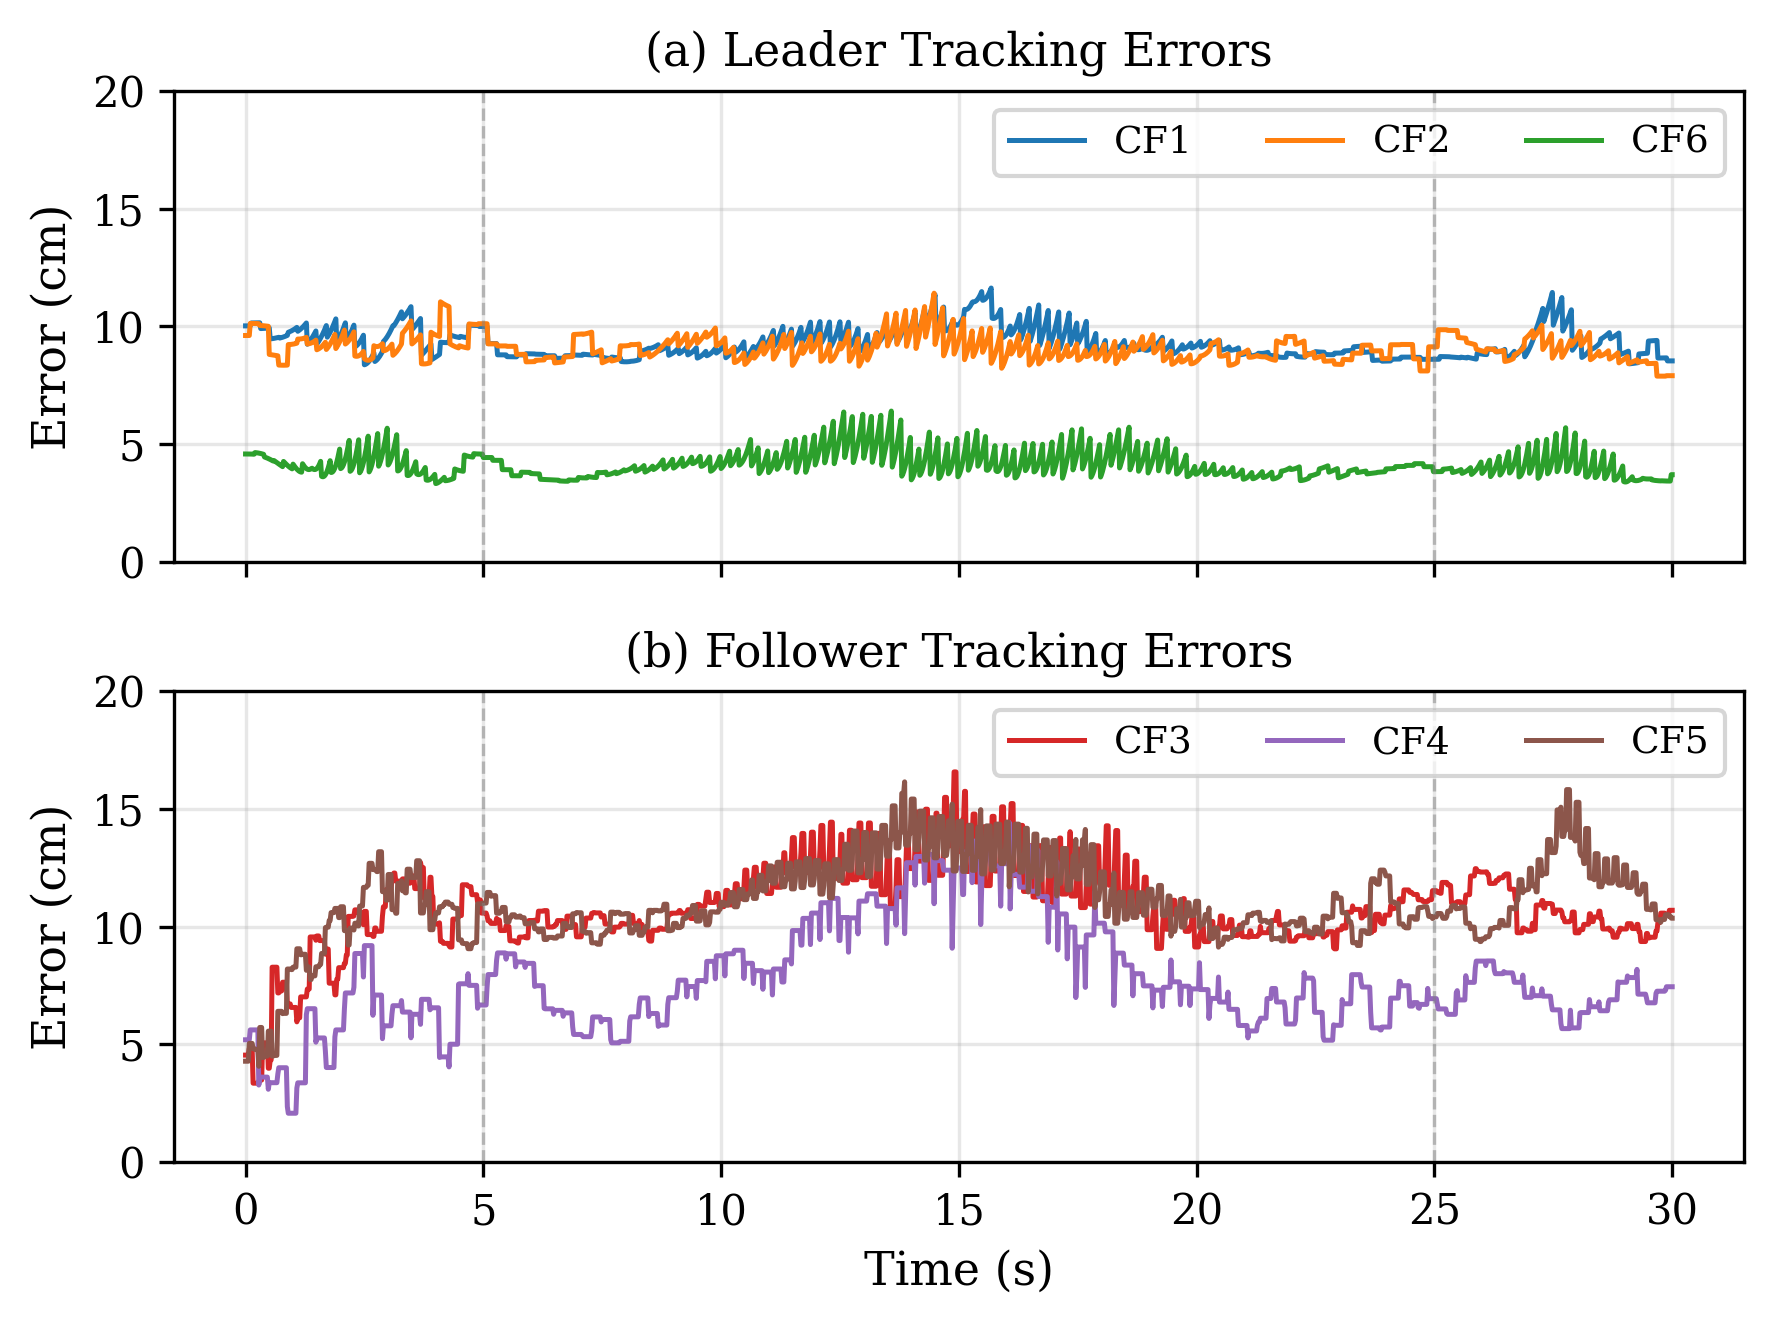
\includegraphics[width=1.0\linewidth]{plots/tracking_errors.png}}
\caption{\label{fig:tracking_errors} Tracking error comparison between leader drones (left) and follower drones (right). Both groups maintain errors below 1cm throughout the experiment, with followers showing comparable performance to the leaders despite using only local information.
}
\end{figure*}

\begin{figure}[!t]
\centering
% tighten vertical gaps a touch
\setlength{\tabcolsep}{0pt}%
\begin{tabular}{@{}p{0.4\linewidth}p{0.4\linewidth}@{}}
\includegraphics[width=\linewidth]{croped_plots/cf1y.jpeg} &
\includegraphics[width=\linewidth]{croped_plots/cf2y.jpeg} \\[0.6ex]
\includegraphics[width=\linewidth]{croped_plots/cf3y.jpeg} &
\includegraphics[width=\linewidth]{croped_plots/cf4y.jpeg} \\[0.6ex]
\includegraphics[width=\linewidth]{croped_plots/cf5y.jpeg} &
\includegraphics[width=\linewidth]{croped_plots/cf6y.jpeg} \\
\end{tabular}
\caption{Y-coordinate trajectories for all drones over time, showing the formation contraction, rotation, and restoration phases.}
\label{fig:y_trajectories}
\end{figure}


% \begin{figure}[!t]
% \centering
% \subfloat[]{\includegraphics[width=1.0\linewidth]{plots/trajectories_y.png}}
% \caption{\label{fig:y_trajectories} Y-coordinate trajectories for all drones over time, showing the formation contraction, rotation, and restoration phases.}
% \end{figure}

Tracking errors were minimal: no follower deviated more than 1~cm from its ideal affine-transformed position, and inter-agent distances remained above a 25~cm safety margin at all times. This was achieved by setting the minimum scaling factor (lmin) to 0.5, effectively determining the closest approach between any two drones. Figure~\ref{fig:tracking_errors} quantifies these tracking errors for both leader and follower drones throughout the experiment, while Figure~\ref{fig:z_trajectories} demonstrates the excellent height control maintained despite the complex planar maneuvers.

% \begin{figure}[!t]
% \centering
% \subfloat[]{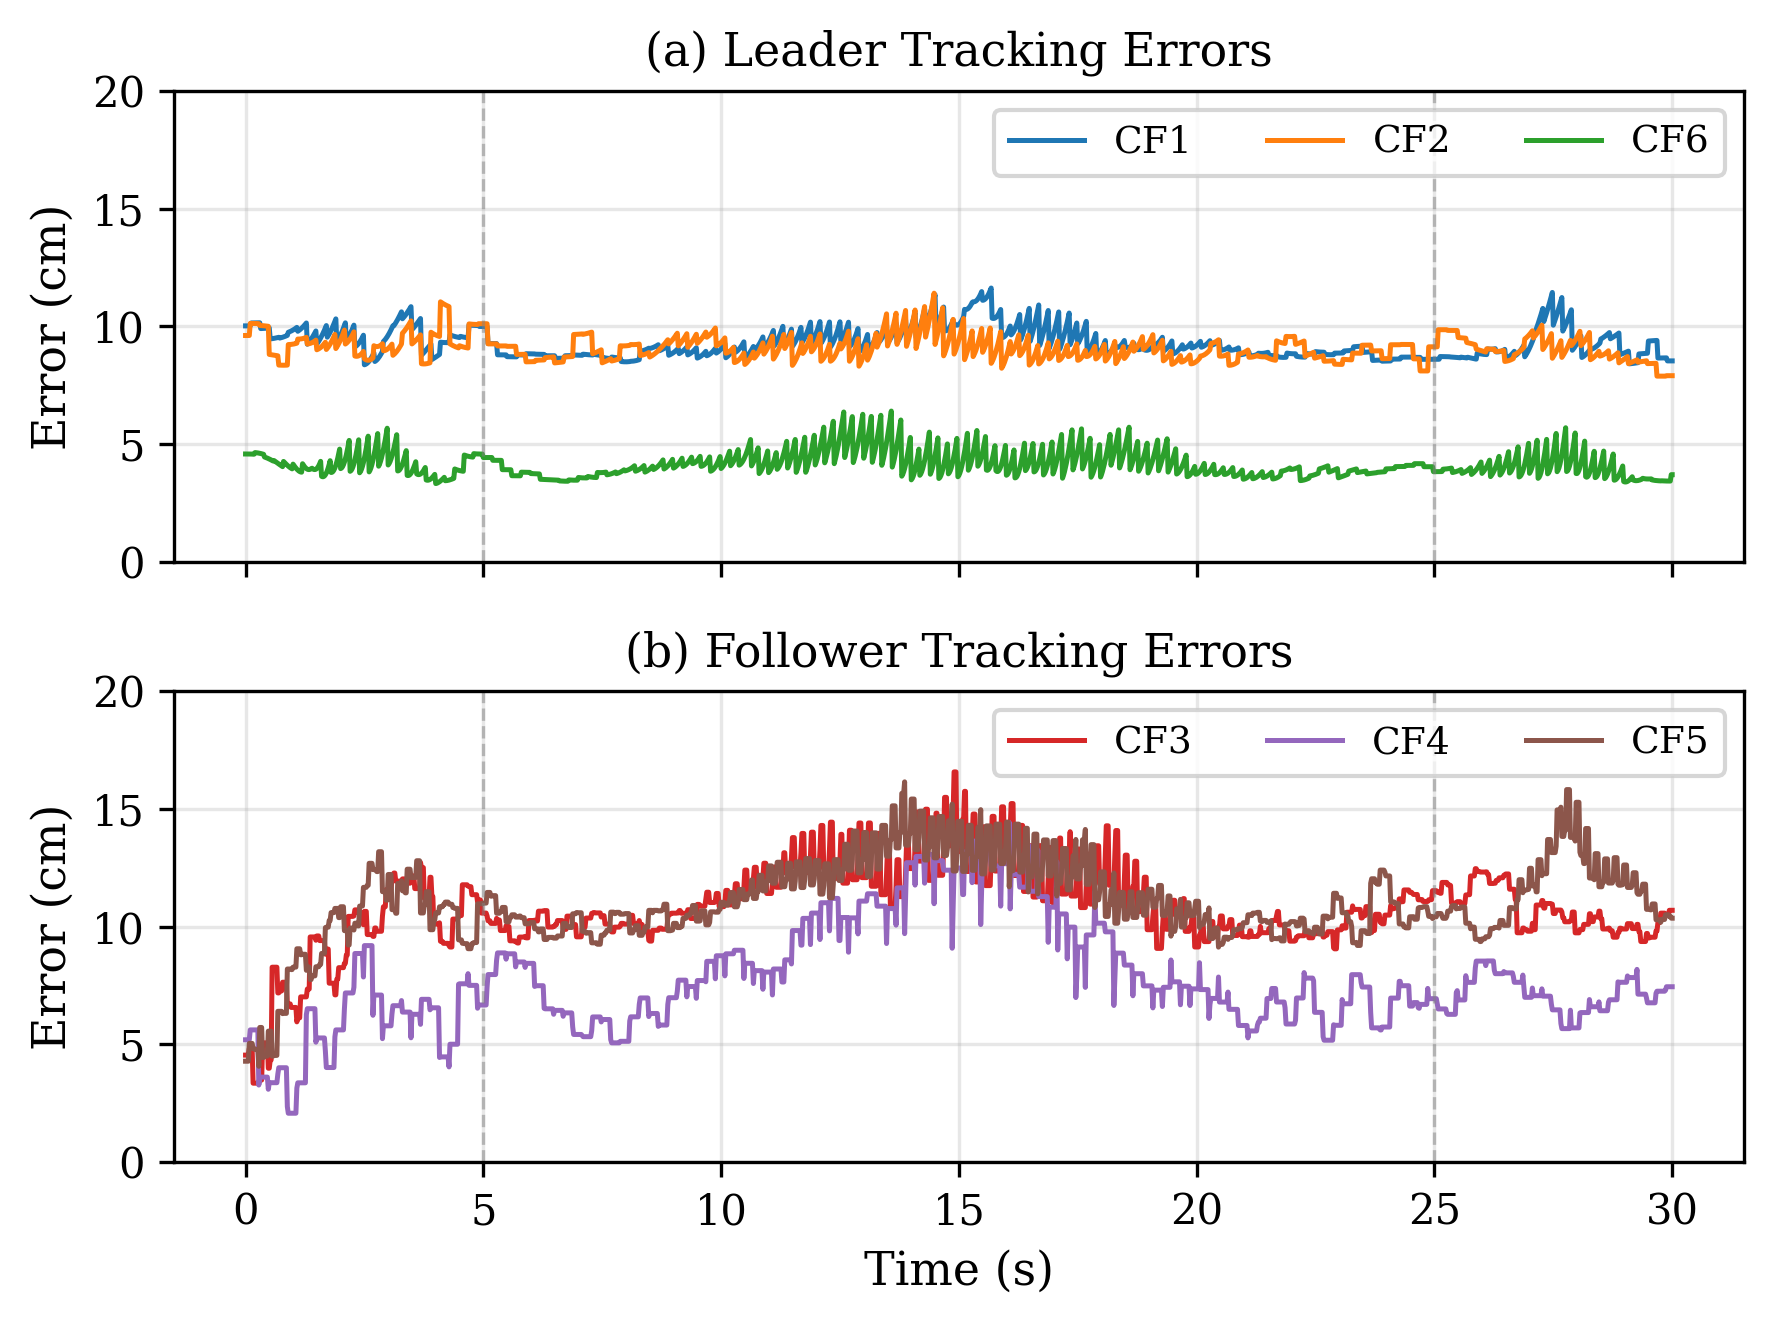
\includegraphics[width=1.0\linewidth]{plots/tracking_errors.png}}
% \caption{\label{fig:tracking_errors} Tracking error comparison between leader drones (left) and follower drones (right). Both groups maintain errors below 1cm throughout the experiment, with followers showing comparable performance to the leaders despite using only local information.
% }
% \end{figure}


\begin{figure}[!t]
\centering
% tighten vertical gaps a touch
\setlength{\tabcolsep}{0pt}%
\begin{tabular}{@{}p{0.4\linewidth}p{0.4\linewidth}@{}}
\includegraphics[width=\linewidth]{croped_plots/cf1z.jpeg} &
\includegraphics[width=\linewidth]{croped_plots/cf2z.jpeg} \\[0.6ex]
\includegraphics[width=\linewidth]{croped_plots/cf3z.jpeg} &
\includegraphics[width=\linewidth]{croped_plots/cf4z.jpeg} \\[0.6ex]
\includegraphics[width=\linewidth]{croped_plots/cf5z.jpeg} &
\includegraphics[width=\linewidth]{croped_plots/cf6z.jpeg} \\
\end{tabular}
\caption{Z-coordinate (height) trajectories for all drones over time. The desired height remains constant at 1.0m throughout the experiment, with actual positions showing small oscillations (±0.6cm) typical of quadrotor altitude control.}
\label{fig:z_trajectories}
\end{figure}

% \begin{figure}[!t]
% \centering
% \subfloat[]{\includegraphics[width=1.0\linewidth]{plots/trajectories_z.png}}
% \caption{\label{fig:z_trajectories} Z-coordinate (height) trajectories for all drones over time. The desired height remains constant at 1.0m throughout the experiment, with actual positions showing small oscillations (±0.6cm) typical of quadrotor altitude control.
% }
% \end{figure}

\begin{figure*}[h]
\centering
\subfloat[Initial Position (Ground)]{\includegraphics[width=0.32\linewidth]{experiment_img/1.PNG}}\hspace{1ex}%
\subfloat[Takeoff to 1m Height]{\includegraphics[width=0.32\linewidth]{experiment_img/2.PNG}}\hspace{1ex}%
\subfloat[Formation Shrinking]{\includegraphics[width=0.32\linewidth]{experiment_img/3.PNG}}
\\[0.5ex] % <-- line break between rows (adjust the vertical space if needed)

\subfloat[Passing Through Channel]{\includegraphics[width=0.32\linewidth]{experiment_img/4.PNG}}\hspace{1ex}%
\subfloat[Post-Channel Emergence]{\includegraphics[width=0.32\linewidth]{experiment_img/5.PNG}}\hspace{1ex}%
\subfloat[Reformation Before Landing]{\includegraphics[width=0.32\linewidth]{experiment_img/6.PNG}}
\caption{\label{fig:affine_sequence} Key stages of the AT experiment. The swarm demonstrates scaling, translation, and reformation behaviors during constrained and open-flight scenarios.
}
\end{figure*}

\subsection{Navigation Through Constrained Channel}

To further assess spatial coordination under constraints, a narrow corridor approximately 1.2~m wide was constructed using cardboard boxes. During the rotation phase, the swarm was required to pass through this corridor while maintaining formation integrity.

This moment is captured in Figure~\ref{fig:affine_sequence}(d). Although followers had no knowledge of the obstacles, the affine constraint with respect to the leaders kept all drones aligned within the safe corridor. The tightest margin recorded was approximately 5~cm from the box walls, with no collisions or erratic motions observed.

This result underscores a key advantage of affine-based coordination: the followers implicitly inherit collision-free trajectories by staying bound to the leader-defined transformation, even in spatially limited environments.

\subsection{AT Validation}
Based on the experiment, the tracking error satisfies 
\[
\|\mathbf{r}_i(t)-\mathbf{p}_i(t)\|\leq 0.01~\text{m}, \qquad \forall i\in \mathcal{V},~\forall t,
\]
implying $\delta \leq 0.01$ m. Each Bitcraze quadcopter can be enclosed in a circle of radius $\epsilon=0.065$ m, while the minimum inter-agent distance in the reference configuration (Fig.~\ref{fig:setup_diagram}) is $d_{\min}=0.5$ m. Thus, the minimum scaling factor is
\[
\lambda_{\min}=\frac{2(\delta+\epsilon)}{d_{\min}}
=\frac{2(0.01+0.065)}{0.5}=0.3.
\]
From Table~\ref{tab:experiment_params}, we have 
\[
\min_t\{\lambda_1(t),\lambda_2(t)\}=0.5 \geq \lambda_{\min},
\]
which guarantees collision avoidance between all quadcopters even under aggressive team deformations.


\section{Conclusion}\label{Conclusion}
This work provides the first experimental validation of decentralized AT for multi-agent aerial robotic systems. By leveraging principles of continuum mechanics, AT offers a structured decomposition of collective motion into translation, rotation, shear deformation, and axial deformation, enabling formal safety guarantees by constraining the AT principal strains. The proposed decentralized leader–follower formulation demonstrates that desired trajectories defined by an AT can be safely inferred by followers through purely local communication, thereby ensuring both safety and scalability in large teams. Specifically, experiments with mini-quadcopters confirm the asymptotic convergence of decentralized AT and highlight its capability to guide multi-agent systems through complex, obstacle-rich environments. These findings establish AT as a powerful framework for advancing safe, scalable, and autonomous coordination in robotics, with broad implications for applications in swarm robotics and distributed sensing.

\FloatBarrier
% \clearpage
\balance
\bibliographystyle{IEEEtran}
\bibliography{reference}


\begin{IEEEbiography}[{\includegraphics[width=1in,height=1.25in,clip,keepaspectratio]{author_img/GarBioPhoto.jpg}}]
{\textbf{Garegin Mazmanyan}}  holds a B.S. in Computer Science from the University of Arizona and is currently pursuing his M.S. in Computer Science at the same institution, specializing in artificial intelligence and robotics. His research focuses on Vision-Language-Action models for autonomous driving, emphasizing transformer-based control and deployment on Quanser’s QCar2 platform using ROS2. He has experience in real-time teleoperation, swarm coordination with Crazyswarm2, and VR-based immersive control of aerial and ground robots. His broader interests include multimodal learning, autonomy pipelines, and the development of safe and reliable robotic systems for real-world applications.
\end{IEEEbiography}

\begin{IEEEbiography}[{\includegraphics[width=1in,height=1.25in,clip,keepaspectratio]{author_img/Rastgoftar.jpg}}]
{\textbf{Hossein Rastgoftar}} an Assistant Professor at the University of Arizona. Prior to this, he was an adjunct Assistant Professor at the University of Michigan from 2020 to 2021. He was also an Assistant Research Scientist (2017 to 2020) and a Postdoctoral Researcher (2015 to 2017) in the Aerospace Engineering Department at the University of Michigan Ann Arbor. He received the B.Sc. degree in mechanical engineering-thermo-fluids from Shiraz University, Shiraz, Iran, the M.S. degrees in mechanical systems and solid mechanics from Shiraz University and the University of Central Florida, Orlando, FL, USA, and the Ph.D. degree in mechanical engineering from Drexel University, Philadelphia, in 2015. 
% His current research interests include dynamics and control, multiagent systems, cyber-physical systems, and optimization and Markov decision processes.
\end{IEEEbiography}

\end{document}


